\documentclass[12pt, a4paper]{article}

\usepackage{tikz}
\usepackage{hyperref}
\usepackage{amsmath}
\usepackage{amssymb}

\title{CAPD-based web application}
\author{Aleksander Pasiut}

\begin{document}
\maketitle

\subsection*{Introduction}
In this project we developed a web interface for a CAPD-based rigorous ODE solver. The application is hosted on a local HTTP server. The user can access the web interface with regular web browser, where they can specify the ODE problem parameters, trigger the computation and read the result. 

\begin{figure}[h!]
    \begin{center}
        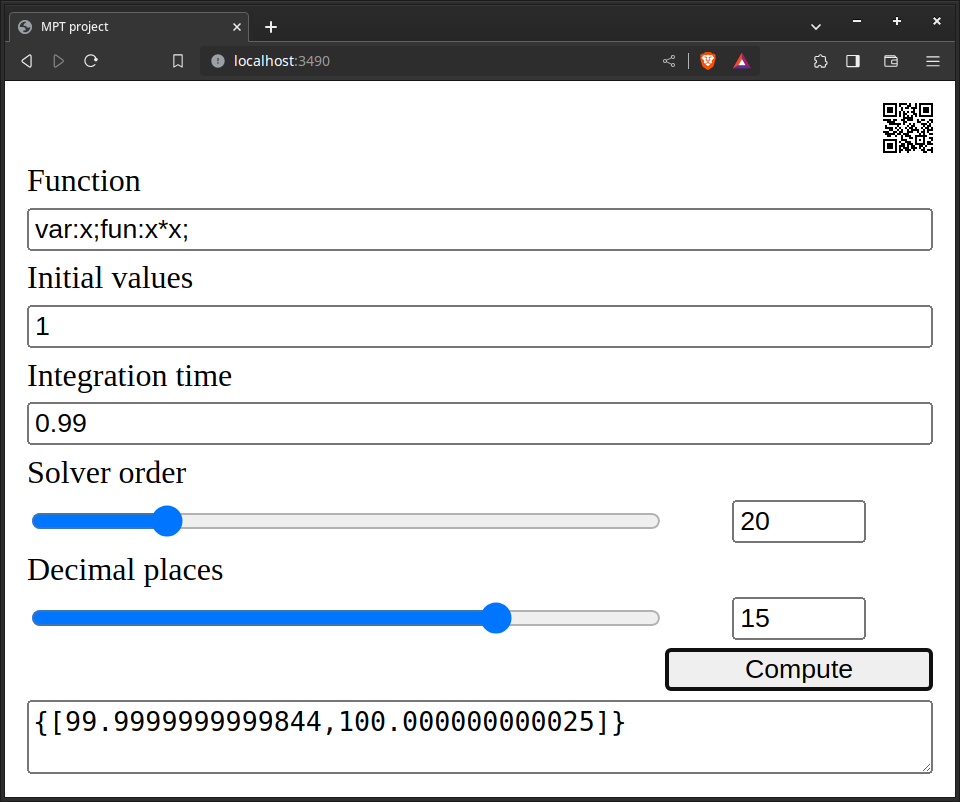
\includegraphics[width=0.85\textwidth]{gui.png}
    \end{center}
    \caption{Screenshot of a web interface.}
    \label{fig:gui}
\end{figure}

Simultaneous access of multiple clients is implemented. The handling of exceptions and errors thrown by the library is implemented. The application features timeout to protect from excessively long computations. For the user's convenience, the QR code containing application URL is presented (this allows quick access from another device connected to the same local network).

\subsection*{Prerequisites}
Implementation of HTTP server and integration to CAPD library is done in C++ programming language (standard C++17). CMake build system is used to automate the compilation and linking. Website interface is written in HTML, CSS and JavaScript. The implementation can be build for Linux operating system only (other operating systems are not supported).

\subsection*{Functionality overview}
The primary functionality of the application is solving ODE equations with rigorous numerical interval computations. Formally, we obtain the interval vector that contains the exact value of the function $x : [0;t] \to \mathbb{R}^N$ at argument $t$, which is the solution of the equation:
\[
    x'(t) = f \left( x(t) \right),
\]
where $f : \mathbb{R}^N \to \mathbb{R}^N$ and $x(0) = x_0$. User specifies the function $f$, initial value $x_0$, integration time $t$, solver order and the number of the decimal places of the result. The decimal separator is dot ".", while the variables and vector components are separated with comma ",".

\subsection*{Architecture}
The figure \ref{fig:architecture} presents the block diagram of main components of the application and their relationships.

\begin{figure}[h]
    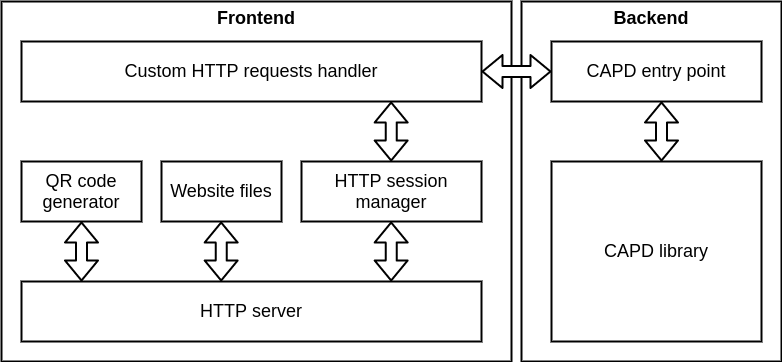
\includegraphics[width=\textwidth]{architecture.png}
    \caption{Block diagram of the primary components of the application}
    \label{fig:architecture}
\end{figure}

The application consists of two executables: Backend and Frontend. The first one is linked to CAPD library (which is build from the source code along with the entire application) and is responsible for passing ODE problem parameters to the solver and returning the result. Frontend component implements HTTP server and manages the Backend component. It is responsible for providing website files, QR code generation, session handling, launching Backend component with specified parameters, retrieving the result, error handling and computation timeout handling.

\subsection*{Links and references}
Application source code is available at \url{ https://github.com/AleksanderPasiut/mpt_project }. The information about CAPD library can be found at \url{ http://capd.ii.uj.edu.pl/ }. We emphasize that this application uses the fork of CAPD library source code, not the official release.

\end{document}
